\chapter{Installation/Benutzung}
\label{cha:Installation/Benutzung}

\section{Deployment Diagramm}

\begin{figure}[hbt]
	\centering
	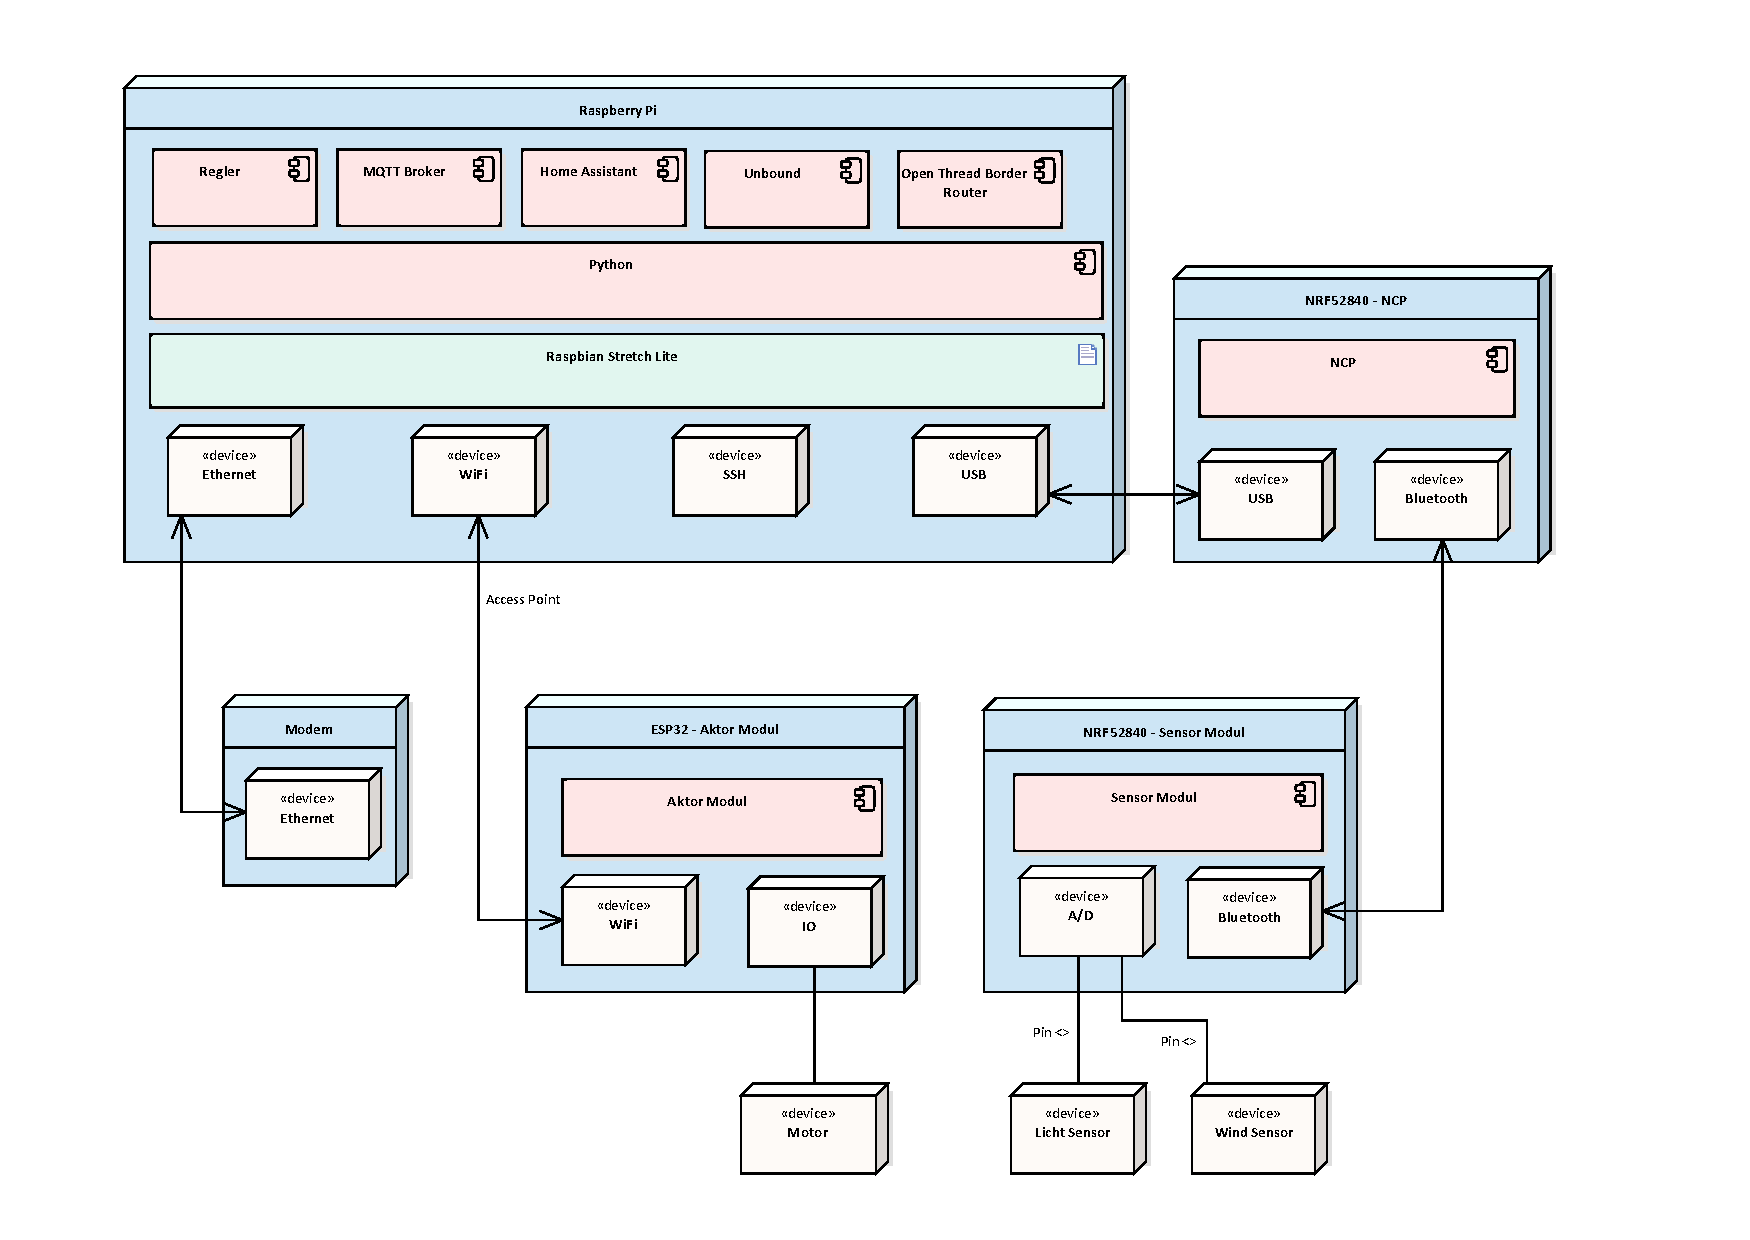
\includegraphics[width=1\linewidth]{images/Deployment}
	\caption[Deployment Diagramm]{Deployment Diagramm.}
	\label{fig:deployment_diagramm}
\end{figure}

Abbildung~\ref{fig:deployment_diagramm} zeigt das Deployment Diagramm des Systems. Im Folgenden wird einzeln auf die Installation der Module eingegangen.

\section{Sensor und Aktor Modul (ESP32)}
\label{cha:Installation_IDF}
\subsection{Schritt 1: Installation der ESP IDF}
Um die ESP32 Mikrocontroller flashen zu können, muss zunächst das Espressif IoT Development Framework (ESP IDF)\nomenclature{ESP IDF}{Espressif IoT Development Framework} installiert und eingerichtet werden. An dieser Stelle sei auf die \href{https://docs.espressif.com/projects/esp-idf/en/latest/index.html}{Dokumentation von Espressif} hingewiesen, um die Programmierumgebung abhängig vom Betriebssystem richtig einzurichten. Weiterhin wird eine Installation von Git, sowie make benötigt.

\subsection{Schritt 2: Anpassung der Konfiguration}
Der Quellcode für beide Module kann auf Github heruntergeladen werden: \href{https://github.com/maxbachmann-university/esp32-sensor-modul}{Sensor Modul}, \href{https://github.com/maxbachmann-university/esp32-actuator-module}{Aktor Modul}.

Zum Flashen des ESP32 gibt es entsprechende Makefiles, die den Vorgang vereinfachen. Einstellungen können mit \textbf{''make menuconfig''} vorgenommen werden. Die Abbildungen~\ref{fig:config_start} und ~\ref{fig:config_default} zeigen das Dialogfenster.
Interessante Einstellungsmöglichkeiten sind hier die Elemente:
\begin{itemize}
	\item \textbf{Security Features} um secure boot, sowie flash encryption zu aktivieren bzw. zu deaktivieren (Diese Einstellung sollte bei Unsicherheit besser deaktiviert bleiben, da sie in der Regel nicht umkehrbar ist)
	\item \textbf{Serial Flasher Config} Hier kann der serielle Port an dem der ESP32 hängt ausgewählt werden
	\item \textbf{Example Configuration} Hier können Projektspezifische Parameter wie die Verbindungsdaten des WLAN Routers, des MQTT Brokers und des OTA Servers angepasst werden
\end{itemize}

Im Folgenden sind die benötigten Befehle zum Flashen des ESP32 sowohl für das Sensor Modul, als auch für das Aktor Modul gelistet.
\lstset{caption={Installation des Sensor Moduls}}
\lstset{label={lst:rc.local}}
\begin{lstlisting}
git clone --depth=1 https://github.com/maxbachmann-university/esp32-sensor-modul
cd esp32-sensor-modul
make menuconfig		# Konfiguration vornehmen
make flash			# Flashen des esp32
\end{lstlisting}

\lstset{caption={Installation des Aktor Moduls}}
\lstset{label={lst:rc.local}}
\begin{lstlisting}
git clone --depth=1 https://github.com/maxbachmann-university/esp32-actuator-module
cd esp32-actuator-module
make menuconfig		# Konfiguration vornehmen
make flash			# Flashen des esp32
\end{lstlisting}

\begin{figure}[hbt]
	\centering
	\includegraphics[width=0.8\linewidth]{images/make_menuconfig_start}
	\caption[Konfiguration Startseite]{Startseite der Konfiguration.}
	\label{fig:config_start}
\end{figure}

\begin{figure}[hbt]
	\centering
	\includegraphics[width=0.8\linewidth]{images/make_menuconfig_default}
	\caption[Konfiguration Standard]{Default Werte der Konfiguration.}
	\label{fig:config_default}
\end{figure}

\section{Regler Modul (Raspberry PI)}

\subsection{Schritt 1: Installation von Raspbian}
Zunächst muss das image der aktuellsten Version von \href{https://www.raspberrypi.org/downloads/raspbian/}{Raspbian} auf die SD-Karte des Raspberry PI geladen werden.

\subsection{Schritt 2: MQTT Broker}
Im Grunde kann ein beliebiger MQTT Broker genutzt werden. Wir haben \href{http://mosquitto.org/}{Mosquitto} benutzt. Dieser Broker kann mit dem Befehl in Listing~\ref{lst:installmosquitto} installiert werden und läuft sofort.

\lstset{caption={Installation von Mosquitto.}}
\lstset{label={lst:installmosquitto}}
\begin{lstlisting}
sudo apt-get install -y mosquitto mosquitto-clients
\end{lstlisting}

\subsection{Schritt 3: Hinzufügen des Python Skripts}
Für die Regelung wird ein \href{https://github.com/maxbachmann-university/blind-controller}{Python Skript} verwendet, welches auch auf Github zu finden ist. Dieses kann in einem beliebigen Ort auf dem Raspberry Pi gespeichert werden, inklusive der ''config.yml'' Datei. In dieser können die Zugangsdaten zu dem MQTT Broker angepasst werden. Für den Autostart des Skripts beim Neustart, muss mit Hilfe des Befehls wie in Listing~\ref{lst:rc.local} im Terminal der Texteditor der Datei ''rc.local'' aufgerufen werden. Anschließend wird die Datei vor der Zeile ''exit 0'' um eine weitere Zeile ergänzt, in die nach einem ''python'' der Pfad zu dem Python Skript angegeben wird, gefolgt von einem ''\&''. Das ganze sieht dann zum Beispiel so aus, wie in Listing~\ref{lst:autostart}.

\lstset{caption={Öffnen der Autostart Datei im Editor Nano.}}
\lstset{label={lst:rc.local}}
\begin{lstlisting}
sudo nano /etc/rc.local
\end{lstlisting}

\lstset{caption={Anpassung der Autostart Datei.}}
\lstset{label={lst:autostart}}
\lstset{language=Python}
\begin{lstlisting}
python3 /home/pi/controller.py &
exit 0
\end{lstlisting}